Multiple choice section. All points are for choosing the correct answer. No justification is needed.
\begin{questions} 
\question[3] The number $i^{7}$ is equal to
\begin{checkboxes}
    \choice $i$
    \choice $-1$
    \choice $-i$
    \choice $1$
    \choice None of the Above
\end{checkboxes}

\question[3] The domain of $\dfrac{1}{\sqrt{x+4}}$ is:
\begin{checkboxes}
    \choice $(-\infty,-4]$
    \choice $(-\infty, -4)$
    \choice $[-4,\infty)$
    \choice $(-4,\infty)$
    \choice $x\ge 0$
\end{checkboxes}

\question[3] Select the correct graph of $f(x)=\left\{\begin{matrix}
    x^2 &,& x\ge 0\\
    2x &,& x<0
\end{matrix}\right.$  
\begin{multicols}{2}
    

\begin{checkboxes}
    \choice \phantom{a}\vspace{-.7cm}
    
    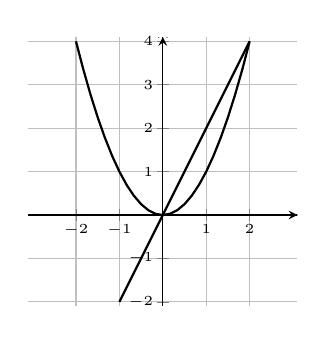
\begin{tikzpicture}%[domain=-4:4]
    \begin{axis}[
    grid=major,
    axis x line = middle,
    axis y line = middle,
        yticklabel style = {font=\tiny,xshift=0.5ex},
        xticklabel style = {font=\tiny,yshift=0.5ex},
    %scale only axis=true,
    width=5 cm,
    height=5 cm,
    xtick={-2,-1,0,1,2},
    ytick={-2,-1,0,1,2,3,4},
    xmin=-3.1,
    xmax=3.1,
    ymin=-2.1,
    ymax=4.1,
    ]
  %\draw[very thin,color=gray] (-2.9,-2.1) grid (2.9,2.9);

  \draw[->] (-4.2,0) -- (4.2,0) node[right] {$x$};
  \draw[->] (0,-1.2) -- (0,4.2) node[above] {$f(x)$};

  \draw[thick, domain=-2:2]    plot (\x,\x*\x) ;%            node[right] {$f(x) =x$};
  % \x r means to convert '\x' from degrees to _r_adians:
  \draw[thick, domain=-1:2]   plot (\x,2*\x) ;%   node[right] {$f(x) = \sin x$};
  %\draw[color=orange] plot (\x,{0.05*exp(\x)}) node[right] {$f(x) = \frac{1}{20} \mathrm e^x$};
  \end{axis}
\end{tikzpicture}

\choice \phantom{a}\vspace{-.7cm}
    
    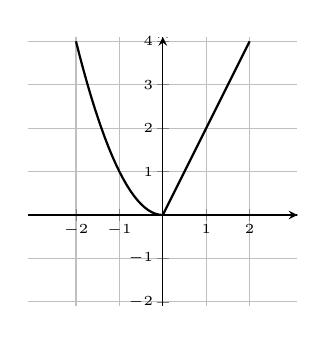
\begin{tikzpicture}%[domain=-4:4]
    \begin{axis}[
    grid=major,
    axis x line = middle,
    axis y line = middle,
        yticklabel style = {font=\tiny,xshift=0.5ex},
        xticklabel style = {font=\tiny,yshift=0.5ex},
    %scale only axis=true,
    width=5 cm,
    height=5 cm,
    xtick={-2,-1,0,1,2},
    ytick={-2,-1,0,1,2,3,4},
    xmin=-3.1,
    xmax=3.1,
    ymin=-2.1,
    ymax=4.1,
    ]
  %\draw[very thin,color=gray] (-2.9,-2.1) grid (2.9,2.9);

  \draw[->] (-4.2,0) -- (4.2,0) node[right] {$x$};
  \draw[->] (0,-1.2) -- (0,4.2) node[above] {$f(x)$};

  \draw[thick, domain=-2:0]    plot (\x,\x*\x) ;%            node[right] {$f(x) =x$};
  % \x r means to convert '\x' from degrees to _r_adians:
  \draw[thick, domain=0:2]   plot (\x,2*\x) ;%   node[right] {$f(x) = \sin x$};
  %\draw[color=orange] plot (\x,{0.05*exp(\x)}) node[right] {$f(x) = \frac{1}{20} \mathrm e^x$};
  \end{axis}
\end{tikzpicture}

\choice \phantom{a}\vspace{-.7cm}
    
    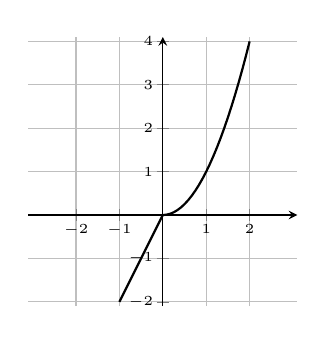
\begin{tikzpicture}%[domain=-4:4]
    \begin{axis}[
    grid=major,
    axis x line = middle,
    axis y line = middle,
        yticklabel style = {font=\tiny,xshift=0.5ex},
        xticklabel style = {font=\tiny,yshift=0.5ex},
    %scale only axis=true,
    width=5 cm,
    height=5 cm,
    xtick={-2,-1,0,1,2},
    ytick={-2,-1,0,1,2,3,4},
    xmin=-3.1,
    xmax=3.1,
    ymin=-2.1,
    ymax=4.1,
    ]

  \draw[thick, domain=0:2]    plot (\x,\x*\x) ;%            node[right] {$f(x) =x$};
  % \x r means to convert '\x' from degrees to _r_adians:
  \draw[thick, domain=-1:0]   plot (\x,2*\x) ;%   node[right] {$f(x) = \sin x$};
  %\draw[color=orange] plot (\x,{0.05*exp(\x)}) node[right] {$f(x) = \frac{1}{20} \mathrm e^x$};
  \end{axis}
\end{tikzpicture}
\choice \phantom{a}\vspace{-.7cm}
    
    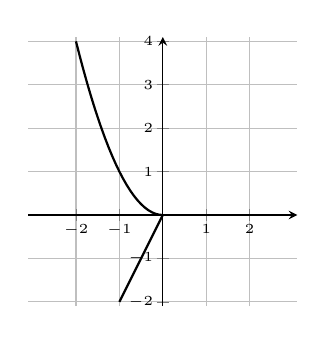
\begin{tikzpicture}
    \begin{axis}[
    grid=major,
    axis x line = middle,
    axis y line = middle,
        yticklabel style = {font=\tiny,xshift=0.5ex},
        xticklabel style = {font=\tiny,yshift=0.5ex},
    width=5 cm,
    height=5 cm,
    xtick={-2,-1,0,1,2},
    ytick={-2,-1,0,1,2,3,4},
    xmin=-3.1,
    xmax=3.1,
    ymin=-2.1,
    ymax=4.1,
    ]

  \draw[thick, domain=-2:0]    plot (\x,\x*\x) ;
  \draw[thick, domain=-1:0]   plot (\x,2*\x) ;
  \end{axis}
\end{tikzpicture}

\end{checkboxes}
\end{multicols}

\newpage
\question[3] Determine whether the curve below represents a function.

\begin{center}

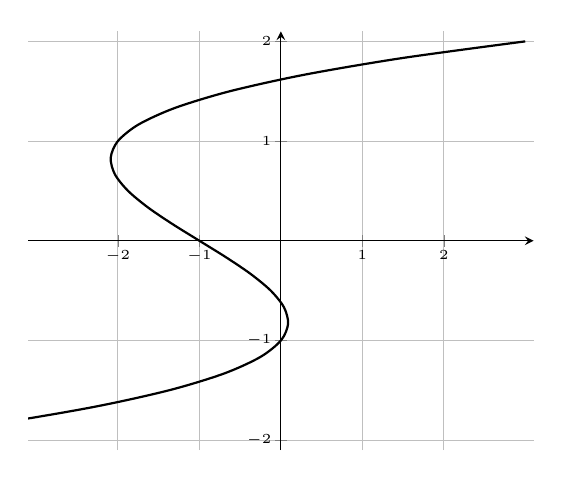
\begin{tikzpicture}
    \begin{axis}[
    grid=major,
    axis x line = middle,
    axis y line = middle,
        yticklabel style = {font=\tiny,xshift=0.5ex},
        xticklabel style = {font=\tiny,yshift=0.5ex},
    width=8 cm,
    %height=5 cm,
    xtick={-2,-1,0,1,2},
    ytick={-3,-2,-1,0,1,2,3,4},
    xmin=-3.1,
    xmax=3.1,
    ymin=-2.1,
    ymax=2.1,
    ]

\draw[thick] plot[variable=\t,domain=-2:2,smooth,thick] (\t*\t*\t-2*\t-1,\t);

  \end{axis}
\end{tikzpicture}
    
\end{center}
\begin{checkboxes}
    \choice Function: The graph passes the horizontal line test.
    \choice Not a Function: The graph fails the horizontal line test.
    \choice Not a Function: The graph fails the vertical line test.
    \choice Function: The graph passes the vertical line test.
    
    \choice We cannot tell from the graph whether or not it represents a function.
\end{checkboxes}

% \question[3] Find the solution set for the following inequality.
% \[ x^2+4x\le 5\]
% \begin{checkboxes}
%     \choice $[-4,0]$
%     \choice $(-\infty,-5]\bigcup [1,\infty)$
%     \choice $[0,5]$
%     \choice $[-5,1]$
%     \choice None of the above.
% \end{checkboxes}

\question[3] Find all \textbf{real} solutions to the following equation.
\[ x^4=9x^2\]
\begin{checkboxes}
    \choice $x=\sqrt{3},\, x=-\sqrt{3}$
    \choice $x=3,\,x=3$
    \choice $x=0,\,x=\sqrt{3},\,x=-\sqrt{3}$
    \choice $x=0,\,x=3,\,x=-3$
    \choice None of the Above.
\end{checkboxes}

\newpage
%     \question[3] Find the domain of the function:
% \[ \dfrac{x-5}{x^2-25}\]
% \begin{checkboxes}
%     \choice $(-\infty, -5)\bigcup(-5,5)\bigcup(5,\infty)$
%     \choice $(-\infty, -5)\bigcup(-5,\infty)$
%     \choice $(-\infty,5)\bigcup(5,\infty)$
%     \choice $(-\infty, -5)\bigcup(5,\infty)$
%     \choice None of the Above.
% \end{checkboxes}


\hspace{-.5in}Free answer section. Work must be shown to get credit for any answer. Partial credit may be given even for incorrect final answers, so show your work.

\question[5] Perform the operation and write the answer as a single polynomial.
%\begin{parts}	
	% \part[4] $4(x^2-x-3)-5x(x^2+3x)=$
	% %$(5x^2-2x+7)-(3x^2+6x-3)$
	% \vspace{1.1in}
	
	% \hrulefill
%	\part[4] 
 \[(3x-5)(x+3)=\]
	%$(x-5)(3x+2)$
%	\vspace{1.1in}
\vfill	
%	\hrulefill
%	\part[4] $(2x+7)^2=$
%	%$(x+3)^2$
%	\vspace{1.1in}
%	
%	%\hrulefill
%\end{parts}

% \question Factor the following polynomials completely.
% \begin{parts}	
% 	\part[4] $2x^3-18x$
% 	%$x^2+5x$
% 	\vspace{1.1in}
	
% 	\hrulefill
% 	\part[4] $10x^2+3x-1$
% 	%$x^2+x-20$
% 	\vspace{1.1in}
	
% %	\hrulefill
% %	\part[4] $8x^3-27y^3$
% %	%$2x^2+x-3$
% %	%\part[1] $8x^3+27$
% \end{parts}
% \clearpage
\question[7] Perform the following operations and simplify. Your final answer should be
written as a single fraction and contain no common factors in the numerator and
denominator.
%\begin{parts}	
%	\part[4] $ \frac{x-2}{2x-6} \cdot\frac{2x^2-6x}{x+4} $
%	%$ \frac{x-1}{x} \cdot\frac{x+1}{x^2-x} $
%	\vspace{1.5in}
%	
%	\hrulefill
%	\part[4] 
 \[\dfrac{x-2}{x^2-9} -\dfrac{1}{5x+15}\]
	%$ \frac{2x}{x^2-3x+2} -\frac{x+1}{x^2+x-6} $
	\vspace{1.7in}
%\end{parts}
\vfill


\newpage

\question Solve the following equations for all solutions. %[Note 1: At least one of the following will have no solution. For that one, write that is has no solution.] (Note 2: there may be more than one solution, and the solutions may be complex).
\begin{parts}

	\part[7] 
	$  \dfrac{1+3x}{x+2}=5 $

\vfill	

% 	\part[5] 
% 	$  2x^2+x-10=0 $

% \vfill
	

	\part[7] $  \sqrt{2x+5}=x+1 $

\vfill	

\end{parts}

\newpage

% \question[5] %
% 	A group of friends rent a vacation house that costs 
%  \$300 
%  per night. At the last minute, 
% two
%  people in the group decide not to go. This raises the  cost per person by 
%  \$5 per night. 
%  How many people \underline{originally} intended to go on the vacation?
% 	\vspace{4in}
	
% 	%\hrulefill


\question Solve the following inequalities.
\begin{parts}	

	\part[6] $3\ge -4x-7 >-7$

 \vfill

	\part[7] $ x^2-21x+20\ge0 $
 \vfill
\end{parts}
%\newpage

\question[7] Solve the following for $x$.

% \begin{parts}

% 	\part[7] 
 $5-3|x+2|=2$
	\vfill
	

	% \part[5] $|2x-5|\le 11$
	% \vspace{2in}

% \end{parts}
\newpage

\question Plot the following points. %3.1
\begin{parts}	
	\part[2] $A(3, 0),\, B(-4,5)$%$,\, (-\frac{5}{2},-1),\, (-3,3)$%(2,-3), (-4,5), (3,0), $(\frac{3}{2},-1)$\\

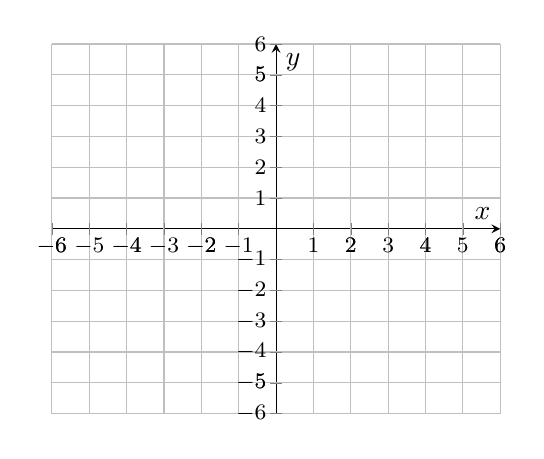
\begin{tikzpicture}
\begin{axis}[
   grid = major,
   extra x ticks={-6,-5,-4,-3,-2,-1,1,2,3,4,5,6},
   extra y ticks={-6,-5,-4,-3,-2,-1,1,2,3,4,5,6},
   %xminorgrids=true,
   width=.6\textwidth,
   %clip = true,
   %clip mode=individual,
   %restrict y to domain=-12:12,
   axis x line = middle,
   axis y line = middle,
        yticklabel style = {font=\footnotesize,xshift=0.5ex},
        xticklabel style = {font=\footnotesize,yshift=0.5ex},
   xlabel={$x$},
   %xlabel style={at=(current axis.right of origin)},
   ylabel={$y$},
   %ylabel style={at=(current axis.above origin)},
   %domain = -5:5,
   xmin = -6,
   xmax = 6,
   %enlarge y limits={rel=0.13},
   %enlarge x limits={rel=0.07},
   ymin = -6,
   ymax = 6,
   %after end axis/.code={\path (axis cs:0,0) node [anchor=north west,yshift=-0.075cm] {0} node [anchor=south east,xshift=-0.075cm] {0};},
 ]
%\draw [thick] plot [smooth, tension=1] coordinates { (-1,0) (0,3) (2,-2) (4,0)};
\end{axis}
\end{tikzpicture}
% \part[3] What is the midpoint of the line segment between $A$ and $B$?
% \vspace{1in}

\part[3] What is the distance between the points $A$ and $B$? (You may leave it as a square root.)
\vfill

\part[3] What is the slope of the line through $A$ and $B$?
\vfill

\part[3] What is an equation of the line through $A$ and $B$?
\vfill
\part[3]
What is the equation of the line through $(2,-3)$ perpendicular to the line through $A$ and $B$
\vfill
\end{parts}

\newpage

% \question Give an equation for the lines described below.
% \begin{parts}	
% 	% \part[3] The line through the points $(4,-1)$, and $(-1,6)$\vspace{1.1in}
	
% 	% \hrulefill
% 	% \part[3] The line with slope $m=-\frac{5}{3}$ through the point (4,-1)\vspace{1.1in}
	
% 	% \hrulefill
% %	\part[3] The line with slope $m=3$ and a $y$-intercept of $b=-4$
% %	\vspace{1in}
% %	
% %	\hrulefill
% 	\part[3] The line through $(4,-7)$ parallel to the line $y=-5x+2$
%  \vspace{1.5in}
	
% %	\hrulefill
% 	\part[3] The line through the point $(-3,8)$ perpendicular to the line $y=7x+1$
%  \vspace{1.5in}
% \end{parts}
\question[8] What is the average rate of change of $f(x)=3x^2-5x$ between $x=-2$ and $x=1$?
\vfill

\question[5] 
%Consider the function $f(x)=\sqrt{12-5x^2+17x}$. 
% Consider the function $f(x)=\sqrt{x+1-2x^2}$. 
Consider the function $f(x)=\sqrt{2x^2-5x}$. 
%\begin{parts}
%    
%
    % \part[3] Find $f(x)$ at $x=-2$.
    % \vspace{2in}
%    
    % \part[4] Solve the above condition to find the domain of the function $f(x)$. Write your answers in interval notation.
    % \vfill
  %  \part[3]
    Let $g(x)=f(-3x)$. 
    
    Write down an expression of $g(x)$. %Write down the domain of $g(x)$ in interval notation. (You do not need to provide any proof.)
    \vfill
%\end{parts}

\newpage

\question Consider the graphs of functions $f(x)$ and $g(x)$ as shown below. (Note: $f$ is a curve, $g$ is straight lines with a corner.)

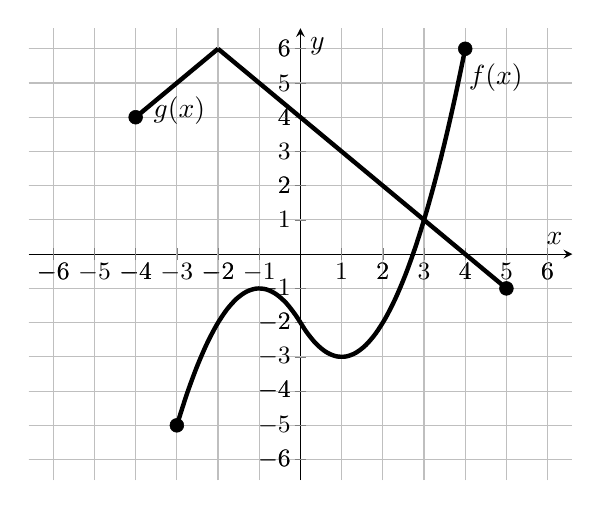
\begin{tikzpicture}
\begin{axis}[
   grid = major,
   extra x ticks={-6,-5,-4,-3,-2,-1,1,2,3,4,5,6},
   extra y ticks={-6,-5,-4,-3,-2,-1,1,2,3,4,5,6},
   %xminorgrids=true,
   width=.7\textwidth,
   %clip = true,
   %clip mode=individual,
   %restrict y to domain=-12:12,
   axis x line = middle,
   axis y line = middle,
        yticklabel style = {font=\small,xshift=0.5ex},
        xticklabel style = {font=\small,yshift=0.5ex},
   xlabel={$x$},
   %xlabel style={at=(current axis.right of origin)},
   ylabel={$y$},
   %ylabel style={at=(current axis.above origin)},
   %domain = -5:5,
   xmin = -6,
   xmax = 6,
   enlarge y limits={rel=0.05},
   enlarge x limits={rel=0.05},
   ymin = -6,
   ymax = 6,
   %after end axis/.code={\path (axis cs:0,0) node [anchor=north west,yshift=-0.075cm] {0} node [anchor=south east,xshift=-0.075cm] {0};},
 ]
     \addplot[domain=-3:4,samples=30,smooth,ultra thick] {x^2*sign(x)-2*x-2} node[pos=.95](endofplotsquare){} ;
\node [right] at (endofplotsquare) {$f(x)$};%

    \addplot[domain=-4:-2,samples=2,ultra thick] {x+8} 
    node[pos=.1] (endofplotsquare){};

\node [right]  at (endofplotsquare)  {$g(x)$};
    \addplot[domain=-2:5,samples=2,ultra thick] {-x+4} node[pos=.9] (endofplotsquare){};

%\node [right]  at (endofplotsquare)  {$g(x)$};
        %\addplot[fill=white,only marks,mark=*, line width=1.0pt, mark size=2.5pt] coordinates{(-1,0)(2,-2)};
        \addplot[only marks,mark=*, line width=0.2pt, mark size=2.5pt] coordinates{(-3,-5)(4,6) (-4,4)(5,-1)};%\addplot[color=yellow,samples=1000,smooth,ultra thick,unbounded coords=jump,no markers] {ln(x)} node[above,pos=1] {$\ln(x)$};
%\draw [thick] plot [smooth, tension=1] coordinates { (-1,0) (0,3) (2,-2) (4,0)};
\end{axis}
\end{tikzpicture}
\begin{parts}
%     \part[2] The domain of $f$
% \vfill
 \part[3] The range of $g$
\vfill
\part[3] Intervals on which $f$ is increasing
\vfill

% \part[2] Intervals on which $g$ is decreasing 
% \vfill

%  \part[2] A local min for $g$ in the interval $(-3,1)$.
% \vfill

 \part[3] A local max for $f$ in the interval $(-2,2)$.
\vfill

%  \part[2] Value(s) of $x$ for which $f(x)=g(x)$
% \vfill

\part[3]  Interval(s) in $x$ for which $f(x)>g(x)$
\vfill

% \part[3]  Interval(s) in $x$ for which $f(x)>g(x)$
% \vfill
%  \part[3] The net change of $g$ on the interval from $x=$ to $x=$
    
\end{parts}
\end{questions}